% #############################################################################
% This is Chapter 3
% !TEX root = ../main.tex
% #############################################################################
% Change the Name of the Chapter i the following line
\fancychapter{The RADAR Dataset}
\label{chap:toolkit}

This section describes the construction and characterization of RADAR, our corpus of open-source agentic applications. We first delimit what counts as an agentic application for the purposes of this study (Section~\ref{sec:defining-agentic}) and enumerate the frameworks that signal agentic intent (Section~\ref{sec:frameworks}). We then describe how candidate repositories are crawled, filtered, and reduced to a curated set of deployed applications (Section~\ref{sec:crawling}), and finally the metadata we extract to characterize each application's structure and security-relevant design (Sections~\ref{sec:dataset-composition}--\ref{sec:extraction-methodology}). We close by stating the dataset's scope and limitations (Section~\ref{sec:limitations}).
 

\section{Defining and Scoping Agentic Applications}
\label{sec:defining-agentic}
 
For the purposes of this study, we define an \emph{agentic application} as any software system that integrates at least one large language model with external tools, memory systems, or retrieval mechanisms in order to plan and execute multi-step tasks. This definition is deliberately broad: it admits the diversity of systems found in practice while remaining concrete enough to be decided programmatically from a repository's code and dependencies.
 
Within this scope, applications differ along the same dimensions that govern their exposure to the risks discussed in Section~\ref{sec:surface}: how much untrusted external data they consume, the sensitivity of the resources their tools can reach, the degree of autonomy the model is granted in selecting subsequent actions, and whether the system can act on its environment or merely generate text. Concretely, these surface as differences in \emph{model integration} (the number and kind of LLM instances, from a single hosted API call to multiple local deployments), \emph{memory mechanisms} (retrieval-augmented generation, persistent stores, conversation history, or knowledge bases), \emph{external capabilities} (the categories and sensitivity of available tools, from read-only queries to file-system access and authenticated third-party calls), and \emph{autonomy} (the extent to which the model, rather than explicit control flow, decides what happens next). The metadata schema in Section~\ref{sec:metadata-format} is designed to make these dimensions measurable.
 
We restrict the study to applications written in Python and JavaScript/TypeScript. These ecosystems host the majority of widely used agent-development frameworks and account for the dominant share of both research prototypes and production deployments, which lets us analyze a large and representative population while keeping static analysis tractable across a single pair of toolchains.

\section{Agentic Frameworks}
\label{sec:frameworks}
 
Identifying agentic applications by keyword alone is unreliable: the term ``agent'' appears in many unrelated projects (user agents, autonomous systems, build agents). We therefore anchor identification on a curated list of agent-development frameworks, SDKs, and integration protocols, on the assumption that a genuine agentic application depends on at least one of them. Table~\ref{tab:frameworks} lists the frameworks we track, grouped by the role they play. We compiled the list from framework documentation, popular repositories, and community resources, and we treat it as an extensible allow-list: adding a framework requires only its import signatures, after which the crawler recognizes dependent repositories automatically.
 
\begin{table}[t]
\centering
\renewcommand{\arraystretch}{1.1}
\setlength{\tabcolsep}{3pt}
\scriptsize
\caption{Agent-development frameworks, SDKs, and protocols used to identify
candidate repositories (Criterion~2).}
\label{tab:frameworks}
\begin{tabular}{@{}>{\raggedright\arraybackslash}p{0.28\columnwidth}
                  >{\raggedright\arraybackslash}p{0.52\columnwidth}
                  >{\raggedright\arraybackslash}p{0.10\columnwidth}@{}}
\toprule
\textbf{Category} & \textbf{Frameworks} & \textbf{Lang.} \\
\midrule
\emph{Orchestration} & 
  LangChain/LangGraph, AutoGen, CrewAI, Agno, LlamaIndex, Mastra,
  Vercel AI SDK, ElizaOS, Bee Agent, Smolagents, Pydantic AI, Haystack,
  OpenAI Agents SDK, Deep Agents JS &
  Py,JS \\
\emph{LLM SDKs} & 
  OpenAI SDK, Anthropic SDK, Google GenAI, Together SDK, Instructor,
  js-agent, CopilotKit &
  Py,JS \\
\emph{Memory \& RAG} & 
  Mem0, Chroma, Weaviate, Qdrant, Pinecone, Zep, PGVector, Milvus &
  Py,JS \\
\emph{Tool Use} & 
  Playwright, Browser-use, Puppeteer, Stagehand, E2B, Composio &
  Py,JS \\
\emph{Protocols} & 
  MCP SDK, FastMCP, A2A SDK &
  Py,JS \\
\bottomrule
\end{tabular}
\end{table}

\section{Repository Crawling and Selection}
\subsection{Github Crawling}

We collect candidate repositories through the GitHub REST search API, querying for repositories that mention ``agent'' and whose primary language is Python, TypeScript, or JavaScript, sorted by star count in descending order:
 
\begin{scriptsize}
\begin{verbatim}
GET /search/repositories?q=agent&sort=stars&order=desc
\end{verbatim}
\end{scriptsize}

Sorting by popularity prioritizes projects that are maintained and used, and therefore more likely to reflect real development practice. 
%Because the GitHub search API returns at most~1{,}000 results per query, we extend coverage by partitioning the search [\emph{e.g.,} across star-count ranges and additional keyword variants such as \texttt{llm}, \texttt{assistant}, \texttt{autonomous} --- describe the exact partitioning you used], yielding $[N_0]$ raw candidate repositories.

\subsection{Selection Criteria}

We retain a candidate only if it satisfies both of the following criteria, each evaluated automatically during crawling:
 
\begin{itemize}
\item \emph{Criterion~1 (Language composition).} At least 70\% of the repository's code is in Python, TypeScript, or JavaScript combined. This excludes documentation-only repositories and projects whose agent code is incidental to a larger codebase in another language.
\item \emph{Criterion~2 (Framework dependency).} The repository imports or declares a dependency on at least one framework in Table~\ref{tab:frameworks}. We check import statements together with dependency manifests (\texttt{requirements.txt}, \texttt{pyproject.toml}, \texttt{package.json}, \texttt{yarn.lock}). This separates genuine agentic software from projects that merely mention ``agent'' in their description.
\end{itemize}

\subsection{Distinguishing Applications from Frameworks}

Criteria~1 and~2 still admit the frameworks themselves and their tutorials, which are not the deployed applications we wish to study. Separating the two is difficult to automate with syntactic rules, since a framework and an application built on it share most of their imports. 

% Framework, in the context of computer science, is defined as a pre-built structure or foundation that provides reusable, generic functionality to help developers build applications more efficiently. Application is defined as a software program designed to help users perform specific, goal-oriented tasks.

% The distinction between framework and application relies on ideas like "inversion of control", the framework calls your code rather than the reverse, or reusability across problem domains. Those criteria work reasonably well when the two things live in separate repos, like Django versus a Django-based blog: the structural code and the code that uses it are cleanly split. Agentic repos usually don't respect that separation. Most of them are a thin orchestration layer built for, and bundled with, one specific agent, the author wrote the plumbing because they needed it for their one use case, and never pulled it out into its own project. The same commit history can honestly be read either way: a framework that happens to ship with a demo, or an application that happens to contain reusable-looking scaffolding.

% Compounding this, agentic-ness itself is a spectrum rather than a binary, it spans autonomy, tool use, and multi-step planning. So a single repo can score as "framework" on one axis and "application" on another simultaneously. It might expose a generic Agent class and a tool registry (framework signals) while also hardcoding a fixed persona, fixed prompts, and one deployment target (application signals). Surface-level patterns like a .run() call are especially unreliable here, because in agent code, the code that defines a capability and the code that merely uses it tend to look almost identical — you need to see whether a class or interface is actually being created and exposed, not just invoked, before the "framework" label is justified.

% There's also a maturity problem. Many of these repos are early-stage, single-author, and unversioned, so the signals that normally resolve the ambiguity in established software — package metadata, a plugin ecosystem, other projects depending on it — simply haven't had time to appear. A repo that's three commits old with a class called Agent could plausibly grow into a framework or stay a one-off script forever, and nothing in the code as it exists today settles which one it currently "is." That's less a flaw in the classification scheme than a real property of a field where most projects are still figuring out what they're going to become.

We therefore classify each remaining repository using an ensemble of three LLM judges. For each repository we extract the top-level README and prompt each model to decide whether the project is \emph{primarily an agentic application} (a system that uses agents to solve a concrete problem) or \emph{an agent framework} (a library for building such systems). We adopt the majority vote across the three : \textit{deepseek-r1}, \textit{llama3.1} and \textit{gpt-5.4-mini}. This guards against any single model's idiosyncratic errors, and we manually review every case in which the three disagree.
 
\begin{quote}\itshape
``Is this repository primarily an \textbf{agentic application} (a system that uses agents to solve a specific problem) or an \textbf{agent framework} (a library for building agentic applications)? Answer with a single label.''
\end{quote}
 
The three judges agreed unanimously on $29,2\%$ of repositories; the remaining $70,8\%$ required manual adjudication. 
For the RADAR dataset, three LLMs (deepseek-r1, llama-3.1, gpt-5.4-mini) each independently classified 1,000 candidate repositories into one of three labels: \emph{application}, \emph{framework}, or, last case scenario, \emph{needs review}. The majority vote across the three determines each repo's final label, and any case without a majority (or flagged for review) gets manually adjudicated.

The open question was: **how much did the three judges actually agree with each other?** This matters because it tells us how much to trust the automated labeling step versus how much weight the manual review step is really carrying.
Figure~\ref{fig:venn} shows the overlap among the three judges' application labels. Inter-rater agreement was $\kappa=0.098$ (Fleiss' $\kappa$), indicating \emph{slight} consensus. % adjust descriptor to the computed value

% ---------------------------------------------------------------------
% TODO: Venn diagram of the three LLM judges' "application" labels, with
% pairwise and three-way overlap counts annotated on the regions.
% ---------------------------------------------------------------------
\begin{figure}[t]
  \centering
  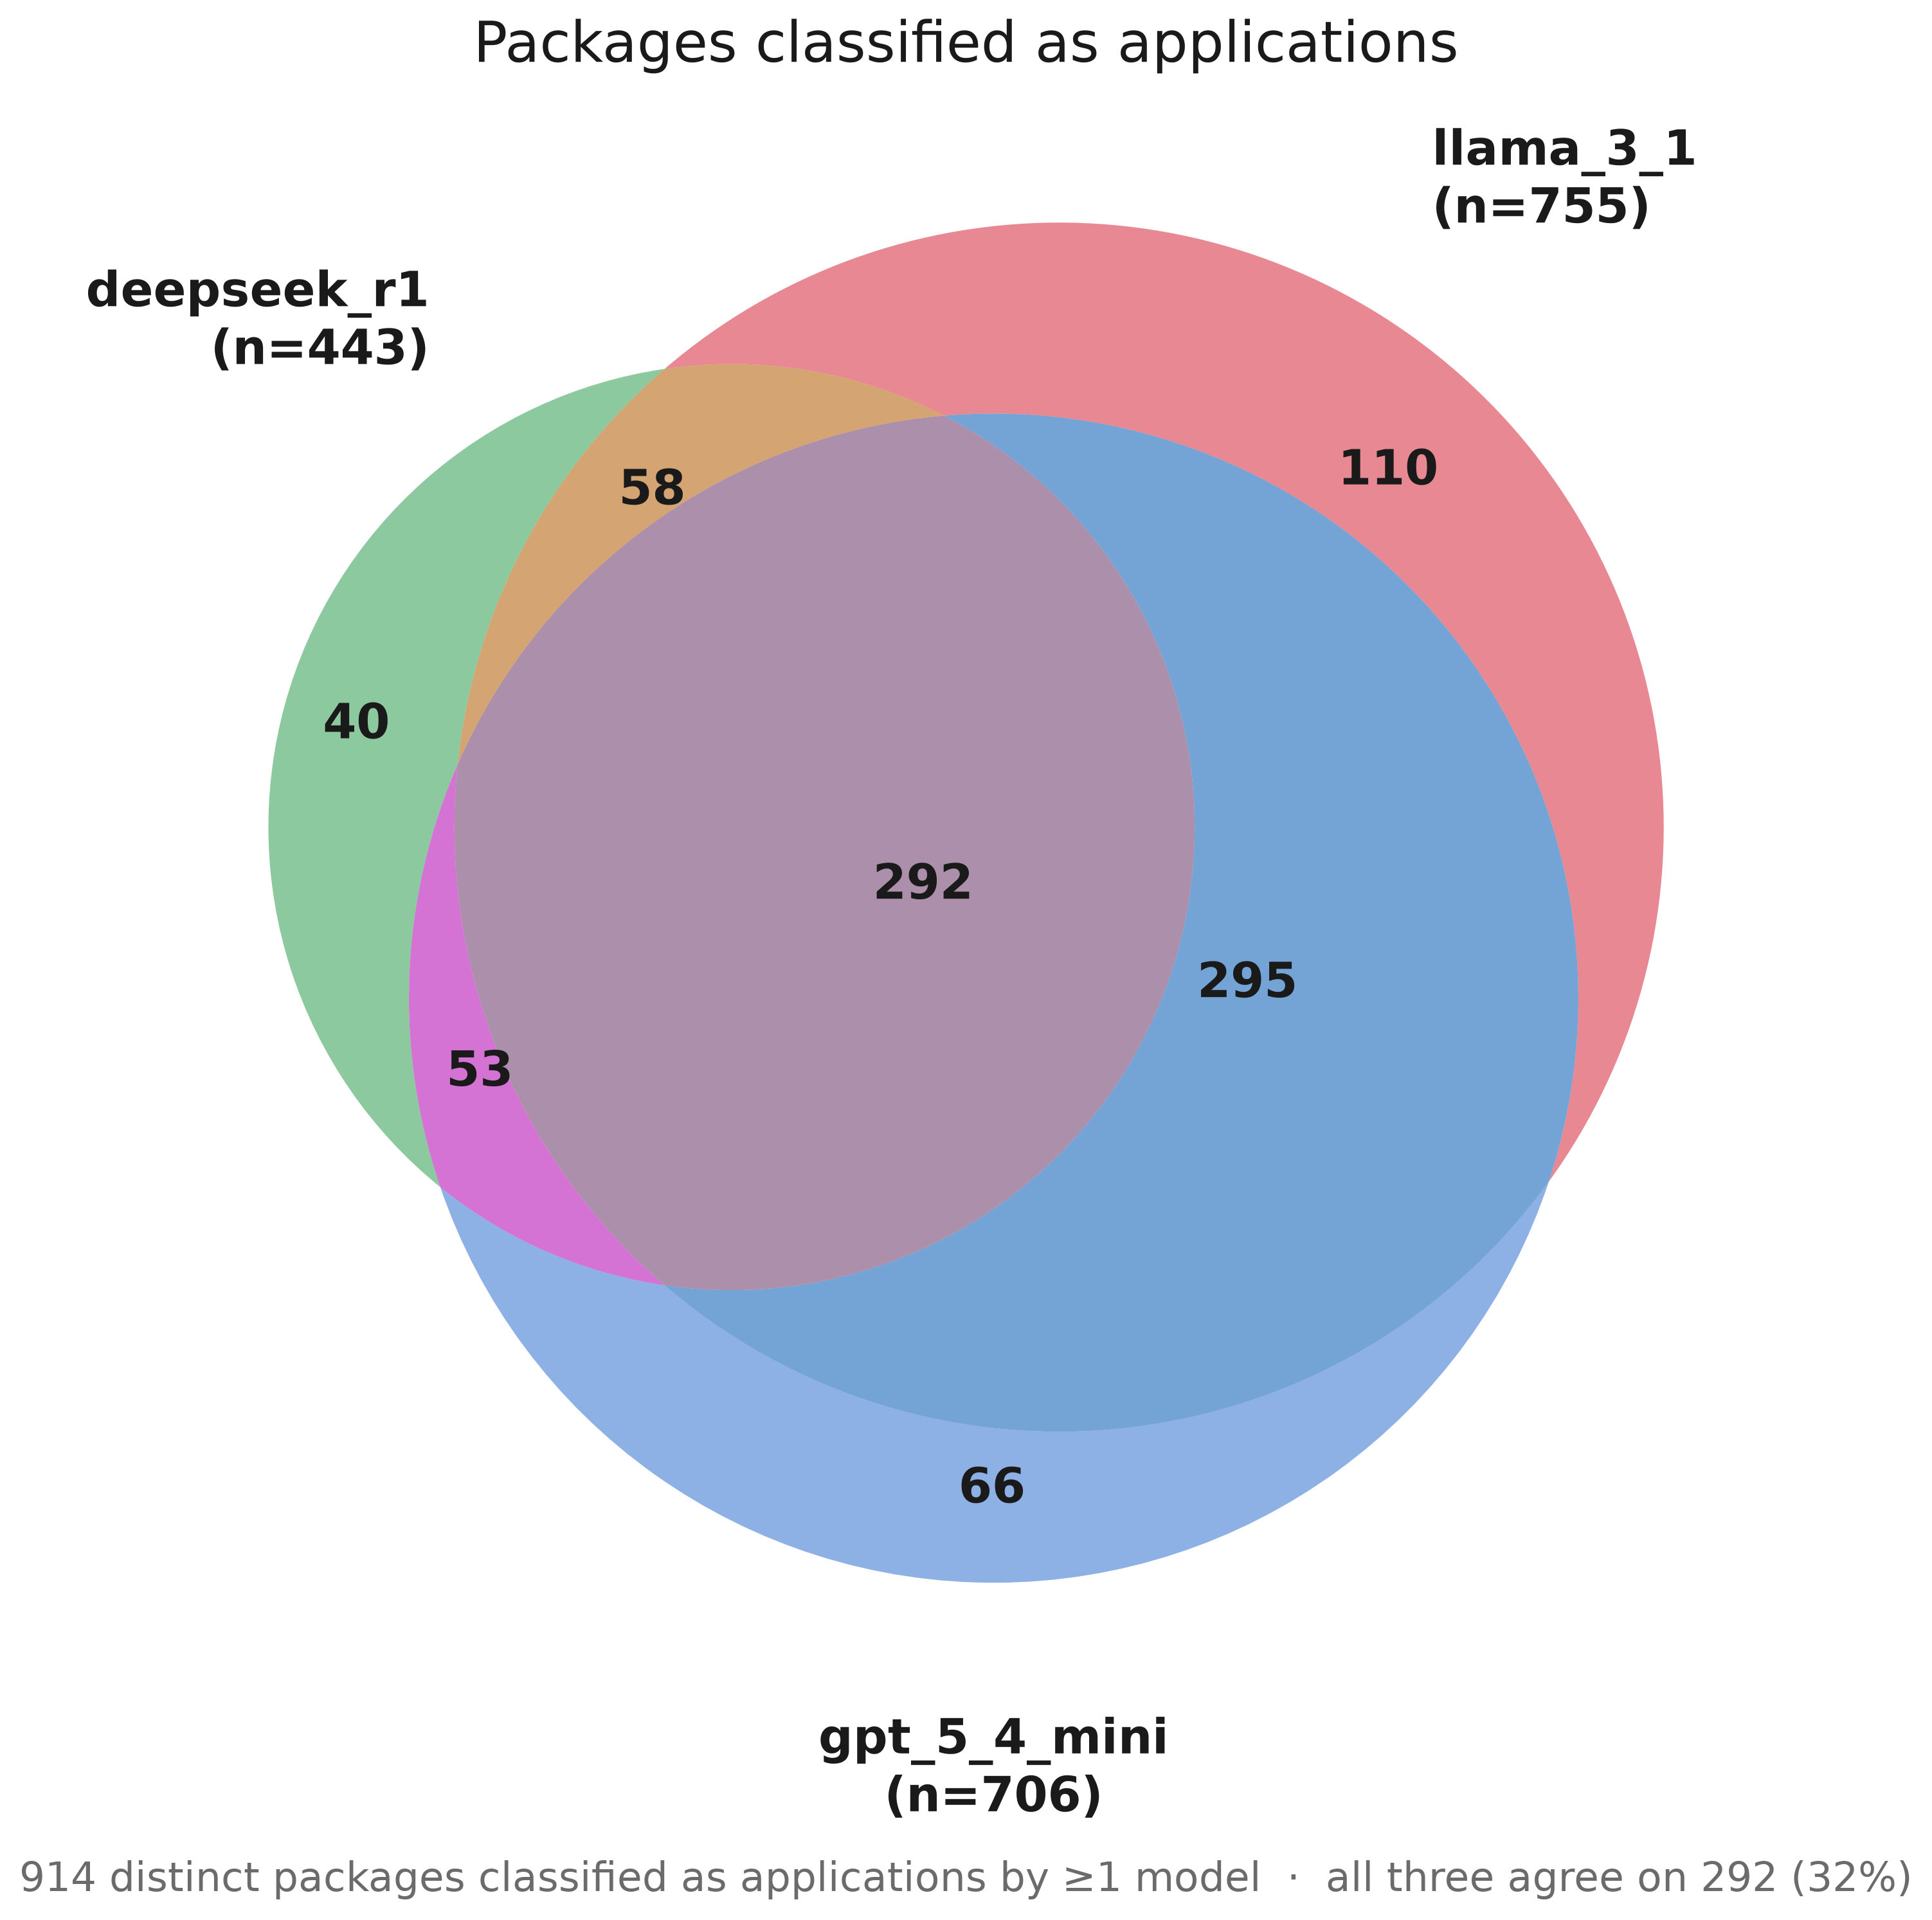
\includegraphics[width=0.8\columnwidth]{Images/venn_applications.png}
  \caption{Overlap of \emph{application} classifications across the three LLM
  judges. Region labels give the number of repositories assigned the
  application label by each subset of judges.}
  \label{fig:venn}
\end{figure}

\subsection{Acquisition Pipeline}

Table~\ref{tab:pipeline} summarizes the full acquisition process, from the raw crawl to the curated dataset.
 
\begin{table}[t]
\centering
\renewcommand{\arraystretch}{1.2}
\setlength{\tabcolsep}{6pt}
\caption{Repository acquisition pipeline. Each stage reports the count
remaining and the number removed.}
\label{tab:pipeline}
\begin{tabular}{@{}>{\raggedright\arraybackslash}p{0.62\columnwidth}rr@{}}
\toprule
\textbf{Stage} & \textbf{Kept} & \textbf{Removed} \\
\midrule
Raw candidates crawled                       & $2034$ & --- \\
Fails Criterion~1 (language composition)     & $1206$ & $828$ \\
Fails Criterion~2 (framework dependency)     & $1000$ & $206$ \\
Classified as not app (excluded)           & $516$ & $484$ \\
\midrule
\textbf{Final RADAR dataset (applications)}  & $\mathbf{516}$ & --- \\
\bottomrule
\end{tabular}
\end{table}

\begin{lstlisting}[language = python, numbers = left, numberstyle = \tiny,
    numbersep = 8pt, escapechar = !,
    basicstyle = \ttfamily\bfseries\footnotesize,
    linewidth = \linewidth,
    frame = tb,
    breaklines = true,
    breakatwhitespace = false,
    caption = {Crawler High-Level Code},
    captionpos = b,
    label = crawler_code]
def crawl_agent_repos(queries, target):
    # Initialize dataset and deduplication store
    dataset = []
    seen = loadSeenRepos()
 
    for query in queries:
        page = 1
        # Fetch repositories page by page, sorted by stars descending
        while page <= MAX_PAGES and len(dataset) < target:
            repos = fetchRepositories(query, page)
 
            # Stop paging once the API returns no more repositories
            if repos == []:
                break
 
            for repo in repos:
                if len(dataset) >= target:
                    break
 
                # Skip repositories already processed in a previous run
                if repo.url in seen:
                    continue
                seen.add(repo.url)
 
                # Selection Criterion 1: language composition
                lang_result = checkLanguages(repo)
                if lang_result.percentage < MIN_LANGUAGE_PERCENTAGE:
                    recordFailure(repo, "language")
                    continue
 
                # Selection Criterion 2: at least one tracked framework
                frameworks = detectFrameworks(repo)
                if frameworks == []:
                    recordFailure(repo, "framework")
                    continue
 
                # Passed both filters: build metadata and store it
                repo_metadata = buildRepoMetadata(repo, lang_result, frameworks)
                dataset.append(repo_metadata)
 
            # Stop paging early if this was the last (partial) page
            if len(repos) < RESULTS_PER_PAGE:
                break
            page += 1
 
    return dataset
\end{lstlisting}


\section{Dataset Composition}

\label{sec:dataset-composition}
 
The final RADAR dataset comprises 516 open-source agentic applications collected from GitHub as of $\text{14/08/2026}$. The corpus spans a range of application domains---including data processing, customer support, software-development assistants, autonomous browser agents, and enterprise automation---and autonomy levels, from user-guided planning to fully autonomous execution. For each application we record the repository metadata listed in Table~\ref{tab:repo-meta}, which captures identifying information together with popularity, maintenance, and scale signals.
 
\begin{table}[t]
\centering
\renewcommand{\arraystretch}{1.2}
\setlength{\tabcolsep}{6pt}
\caption{Repository-level metadata recorded for each application.}
\label{tab:repo-meta}
\begin{tabular}{@{}>{\raggedright\arraybackslash}p{0.42\columnwidth}
                  >{\raggedright\arraybackslash}p{0.46\columnwidth}@{}}
\toprule
\textbf{Field} & \textbf{Description} \\
\midrule
Name, URL, creation date          & Identifying information \\
Stars, forks, last commit         & Popularity \& maintenance \\
Primary language                  & Python / JavaScript / mixed \\
Agent framework(s)                & Framework dependency \\
File count, code size             & Scale of the application \\
Documentation presence            & Project completeness \\
\bottomrule
\end{tabular}
\end{table}
 
The dataset has a median repository size of $415$ files and $1809.8$\,KB of code and a median of $2519.0$ stars (range $14$--$230503$). Framework usage is led by OpenAI SDK ($59,1\%$) and MCP SDK ($45.0\%$), with the remainder split across other frameworks and custom integrations; the distribution of primary use cases is reported in [Figure/Table ref].

\begin{figure}[h]
    \centering
    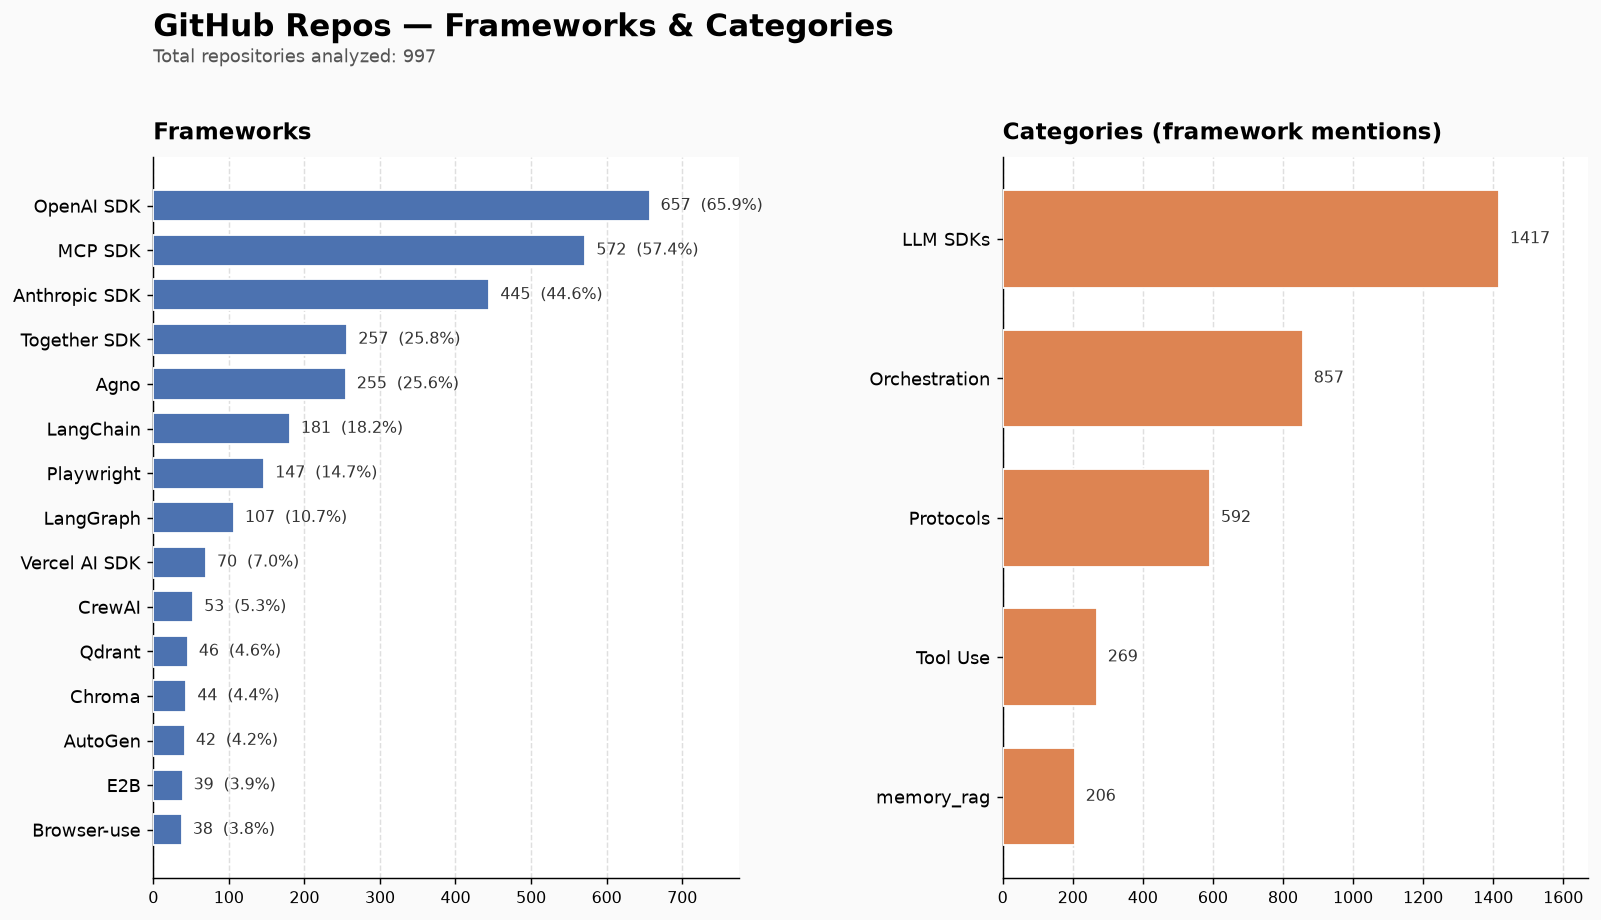
\includegraphics[width=\linewidth]{Images/framework_summary.png}
    \caption{Framework and category frequency across the analyzed
             repositories ($N = 516$). The top panels show absolute
             counts; the bottom table reports percentages of repositories
             (frameworks) and of total framework mentions (categories).}
    \label{fig:framework-summary}
\end{figure}


% #############################################################################
% \section{Agentic Frameworks}

% To identify multi-agent systems in open-source repositories, we first curated a comprehensive list of frameworks commonly used for deploying AI agents. These frameworks fall into three main categories:

% \textbf{Agent Orchestration \& Multi-Agent Systems:} Frameworks that provide native support for creating, coordinating, and managing multiple agents. This category includes LangChain, LangGraph, AutoGen, CrewAI, Agno, and LlamaIndex.

% \textbf{LLM SDKs \& Function Calling:} Frameworks that enable LLM integration and tool/function calling capabilities, including the OpenAI SDK and Anthropic SDK.

% \textbf{Integration Protocols:} Protocols for agent-to-agent communication and tool integration, such as MCP (Model Context Protocol) and A2A (Agent-to-Agent).

% These frameworks were identified through manual inspection of documentation and popular repositories, as well as automated scanning of \texttt{requirements.txt}, \texttt{README.md}, and \texttt{package.json} files.

% \begin{itemize}
%     \item \textbf{package.json}
%  The file is fetched via GitHub's contents API and parsed with parse\_package\_.json. The resulting dependency names are passed to detect\_frameworks\_from\_dependencies(), which loops over every framework in FRAMEWORKS and checks if any of that framework's dependencies strings appear as a key in the parsed dict. First matching dependency string per framework wins (break), so one framework can't be double-counted from the same file. If anything is found, it's returned immediately — requirements.txt and README aren't checked.

%     \item requirements.txt Tried if package.json gave nothing. Same mechanism, but dependencies is now a set/list rather than a dict, so detect\_frameworks\_from\_dependencies takes the list-membership branch (if dep in dependencies) instead of dict-key lookup.

%     \item\textbf{README.md} Only tried if both dependency files are missing or empty. detect\_frameworks\_from\_text() lowercases the whole README and does a substring search for each framework's keywords list. First keyword hit per framework wins, then moves to the next framework.
% \end{itemize}



% \section{Crawler}
% In this section, we explain how we implemented a crawler to collect packages from GitHub that fulfill certain criteria and are representative of real-world multi-agent systems.

% \subsection{Design}

% The crawler utilizes the GitHub REST API to search for repositories that match specific keywords related to agentic applications. The primary search query targets repositories containing code in Python, TypeScript, or JavaScript, as these are the dominant languages for agent development. The results are sorted by number of stars in descending order, ensuring that the most popular and presumably most representative repositories are prioritized.

% % In your lstlisting:
% % \begin{lstlisting}[language = bash, numbers = none, escapechar = !,
% %     basicstyle = \ttfamily\bfseries\footnotesize,  % smaller font helps
% %     linewidth = \linewidth,  % use full width
% %     breaklines = true,
% %     breakatwhitespace = false,  % can break anywhere in URL
% %     caption={GitHub API Search Query}, captionpos=b, label=github_api] 
% %   https://api.github.com/search/repositories?q=agent+language:Python+language:JavaScript&sort=stars&order=desc
% % \end{lstlisting}

% \url{https://api.github.com/search/repositories?q=agent&sort=stars&order=desc}

% To ensure that collected repositories are relevant to our study of multi-agent systems, we applied two additional selection criteria:

% \begin{itemize}
% \item \textbf{Criterion 1: Language Composition.} The repository must consist of at least 70\% code in Python, TypeScript, or JavaScript combined. This ensures that the repository is primarily written in languages commonly used for agent development.

% \item \textbf{Criterion 2: Framework Usage.} The repository must import or depend on at least one of the agent frameworks listed in Section 4.1. This ensures that the repository is genuinely an agentic application rather than a generic software project.
% \end{itemize}

% \begin{lstlisting}[language = javascript, numbers = none, escapechar = !,
%     basicstyle = \ttfamily\bfseries\footnotesize,  % smaller font helps
%     linewidth = \linewidth,
%     frame = tb,
%     breaklines = true,
%     breakatwhitespace = false,
%     caption = {Selection Criteria High-Level Code}, 
%     captionpos = b,
%     label = selection_criteria] 
% {
%   "repo_metadata": {
%     "name": "bytedance/deer-flow",
%     "url": "https://github.com/bytedance/deer-flow",
%     "stars": 63423,
%     "primary_language": "Python",
%     "language_percentages": {...},
%     "total_files": 893,
%     "frameworks": [
%       {"name": "LangChain", "category": "agent_orchestration"},
%       {"name": "LangGraph", "category": "agent_orchestration"},
%       {"name": "Agno", "category": "agent_orchestration"},
%       {"name": "OpenAI SDK", "category": "llm_sdks"},
%       {"name": "Anthropic SDK", "category": "llm_sdks"},
%       {"name": "MCP SDK", "category": "protocols"}
%     ]
%   }
% }
% \end{lstlisting}

% % #############################################################################



% \begin{lstlisting}[language = python, numbers = none, escapechar = !,
%     basicstyle = \ttfamily\bfseries\footnotesize,  % smaller font
%     linewidth = \linewidth,  % CHANGE from .7 to full width
%     frame = tb,
%     breaklines = true,
%     breakatwhitespace = false,
%     caption = {Crawler High-Level Code}, 
%     captionpos = b,
%     label = crawler_code] 
% def crawl_agent_repos():
%     dataset = []
%     while True:
%         repos = fetch_from_github_api()
%         if not repos:
%             break
%         for repo in repos:
%             lang_percent = repo.python_percent + repo.ts_percent + repo.js_percent
%             if lang_percent >= 70:
%                 if has_agent_framework(repo):
%                     metadata = extract_metadata(repo)
%                     dataset.append(metadata)
%     return dataset
% \end{lstlisting}

% \section{Project Metadata Format}
% \begin{center}
% \centering
% \begin{lstlisting}[language = javascript, numbers = none, escapechar = !,
%     basicstyle = \ttfamily\bfseries\footnotesize,
%     linewidth = \linewidth,  % CHANGE from .6 to full width
%     frame = tb,
%     breaklines = true,
%     breakatwhitespace = false,
%     caption = {Project Metadata Format}, 
%     captionpos = b,
%     label = metadata_format] 
% {
%   "structure_metadata": {
%     "n_agents": 3,
%     "n_tools": 8,
%     "has_rag": true,
%     "has_agent_handoffs": true
%   },
%   "rag_metadata": {
%     "shared_across_agents": true,
%     "rag_writers": ["file_upload_agent"],
%     "rag_readers": ["assistant_agent", "deploy_agent"],
%     "unsanitized_writes": true,
%     "rag_influences_actions": true
%   }
% }
% \end{lstlisting}

% \end{center}
% % \end{minipage}

% \subsection{Structure Metadata}

% Structure metadata captures high-level architectural characteristics of the multi-agent system:

% \begin{itemize}
% \item \texttt{n\_agents}: The total number of agent instances created in the codebase. This indicates the scale of the multi-agent system.
% \item \texttt{n\_tools}: The number of tool or function definitions available to agents. Tools represent the actions agents can perform.
% \item \texttt{has\_rag}: A boolean indicating whether the system uses Retrieval-Augmented Generation, which is a prerequisite for RAG-based contamination attacks.
% \item \texttt{has\_agent\_handoffs}: A boolean indicating whether one agent can call or delegate tasks to another agent, representing an alternative contamination path.
% \end{itemize}

% \subsection{RAG Metadata}

% The RAG metadata category is the core contribution of this thesis, as it captures the patterns that enable cross-agent contamination through shared vector databases:

% \begin{itemize}
% \item \texttt{shared\_across\_agents}: A boolean indicating whether the same vector database instance is used by multiple agents. This is the primary prerequisite for cross-agent contamination.
% \item \texttt{rag\_writers}: A list of agents that can add or upsert content to the RAG database. These represent potential contamination sources.
% \item \texttt{rag\_readers}: A list of agents that query or read from the RAG database. These represent potential contamination victims.
% \item \texttt{unsanitized\_writes}: A boolean indicating whether agent writes to RAG occur without input validation or sanitization. When true, the attack is trivially exploitable.
% \item \texttt{rag\_influences\_actions}: A boolean indicating whether RAG content affects agent behavior (tool selection, planning, decisions) rather than just response content. Behavioral contamination is significantly more dangerous than output-only contamination.
% \end{itemize}

% \section{Classification}
% \subsection{}
% We noted that a substantial number of repositories were not necessarily applications but frameworks used to build applications. 
% The goal of this classification step was to differentiate the applications from the frameworks, which proved to be a complex task. We defined a framework as any tool, plugin, or layer that aids in the development of applications. Moreover, applications are defined as any finished products that could be used with a specific objective in mind and that any user can use without previous coding knowledge. Frameworks have a more open-ended use as opposed to applications which usually have one final goal.
% As you will note, in the following sections this classification is not as black and white as one would assume, both for LLMs and by human verification.


% \subsection{}
% In order to filter out the frameworks, we decided to use three different LLMs to classify the repositories by prompting them with the readmes obtained through the Github API. 

% The following prompt was used: 

% If the three LLM judges (llama-3.1, deepseek-r1 and gtp-5.4-mini) agreed unamimously on the classification, application or framework, the repository was automatically classified. As seen in the prompt, the LLM had a third option needs$_$review. This was presented as a last case scenario to the models but still was a possibility.

% We first ran 1,000 repositories through these models, the results are presented in the table bellow.

% The non unanimous votes were viewed manually.
% If the classification was unclear, we took into account whether there was any UI present and the setup is relatively easy with minimal configuration.
% Each repo could fall into a spectrum between framework and application.
% The main issue is that our objective was to sort the repositories into one of two categories, application or framework. When in reality it would fall somewhere in between. We considered the following characteristics to be considered a application: A repo that has a UI but is used for something that could be considered a middle ground and not an end. For example, applications that analyse LLM metrics and usage or apps used for creating graphics to facilitate analysis by humans.